\documentclass[12pt, a4paper, UTF8, fontset=windows]{ctexbook}
\usepackage{amsmath, amsthm, amssymb, amsfonts, bm, color, fancyhdr, framed, geometry, graphicx, hyperref, lastpage, listings, mathrsfs, xcolor}


\linespread{1.5}
\definecolor{shadecolor}{RGB}{241, 241, 255}
\newcounter{problemname}
\newenvironment{problem}{\begin{shaded}\stepcounter{problemname}\par\noindent\textbf{Q\arabic{problemname}.}}{\end{shaded}\par}
\newenvironment{solution}{\par\noindent\textbf{Ans.}}{\par}

\geometry{left=20mm,right=20mm, top=20mm, bottom=22mm} % 页边距
\setlength{\headheight}{15pt}
\pagestyle{fancy} % 设置页脚页眉
\rhead{Assignment2} % 页眉右边
% \noindent % 取消首段缩进

\definecolor{mygreen}{rgb}{0,0.6,0}
\definecolor{mygray}{rgb}{0.5,0.5,0.5}
\definecolor{mymauve}{rgb}{0.58,0,0.82}
% 代码设置
\lstset{ 
backgroundcolor=\color{white},      % choose the background color
basicstyle=\footnotesize\ttfamily,  % size of fonts used for the code
columns=fullflexible,
tabsize=4,
breaklines=true,               % automatic line breaking only at whitespace
captionpos=b,                  % sets the caption-position to bottom
commentstyle=\color{mygreen},  % comment style
keywordstyle=\color{blue},     % keyword style
stringstyle=\color{mymauve}\ttfamily,  % string literal style
frame=single,
rulesepcolor=\color{red!20!green!20!blue!20},
language=c++,
xleftmargin=3em,
xrightmargin=3em
}


\begin{document}

\cfoot{\thepage\ / \pageref{LastPage}} % 页眉中间位添加内容:页码/总页码

\thispagestyle{empty}

\begin{figure}[t]
    \centering
    
\includegraphics[width=6cm]{../../src/images/logo.jpg}
\end{figure}

\vspace*{\fill}
    \begin{center}
        \Huge\textbf{Assignment2}
    \end{center}
\vspace*{\fill}

\begin{table}[b]
    \centering
    \large
    \begin{tabular}{ll}
    \textbf{课程:} & 算法设计与分析 \\
    \textbf{姓名:} & 雷翔 \\
    \textbf{学号:} & 2053932 \\
    \textbf{时间:} & 2023年4月 \\
    \end{tabular}
\end{table}


\newpage

\setcounter{page}{1} % 页码从当前页开始

\begin{problem}
    请估计一下,对于一个包含 1000000 个元素的有序数组进行成功查找,折半查找比顺序查找平均快多少倍?
\end{problem}

\begin{solution}
    前提:成功查找

    顺序查找的平均查找长度:
    $$ASL_1 = \frac{1 + 2 + ··· + n}{2} = \frac{n+1}{2} = 500000.5$$ 

    折半查找的平均查找长度:
    $$ASL_2 = \lfloor \log_{2}{n} \rfloor + 1 = \lfloor \log_{2}{1000000} \rfloor + 1 = 20$$ 

    折半查找比顺序查找平均快 500000.5/20 = 25000.025 倍 

    % \vspace{2mm}  % 指定高度,添加空行
\end{solution}

% \newpage

\begin{problem}
    N 个士兵组成的小分队必须越过一条又深又宽又没有桥的河。他们注意到在岸旁有两个 12 岁大的小男孩在玩划艇。然而船非常小,只能容纳两个男孩或者一名士兵。 怎样才能让士兵渡过河并且留下两个男孩共同操纵这条船?这条船要在岸与岸之间渡多少次?
\end{problem}

\begin{solution}
    符号说明: 

    $C_i$:第 $i$ 个孩子

    $S_j$:第 $j$ 个士兵

    首先考虑只有一个士兵的情况,两个孩子首先把船划到对岸,再由其中一个孩子把船划回来,士兵再把船划到对岸,再对岸的孩子把船划回来,所以让一个士兵渡过河需要4次。

    \begin{figure}[h]
        \centering
        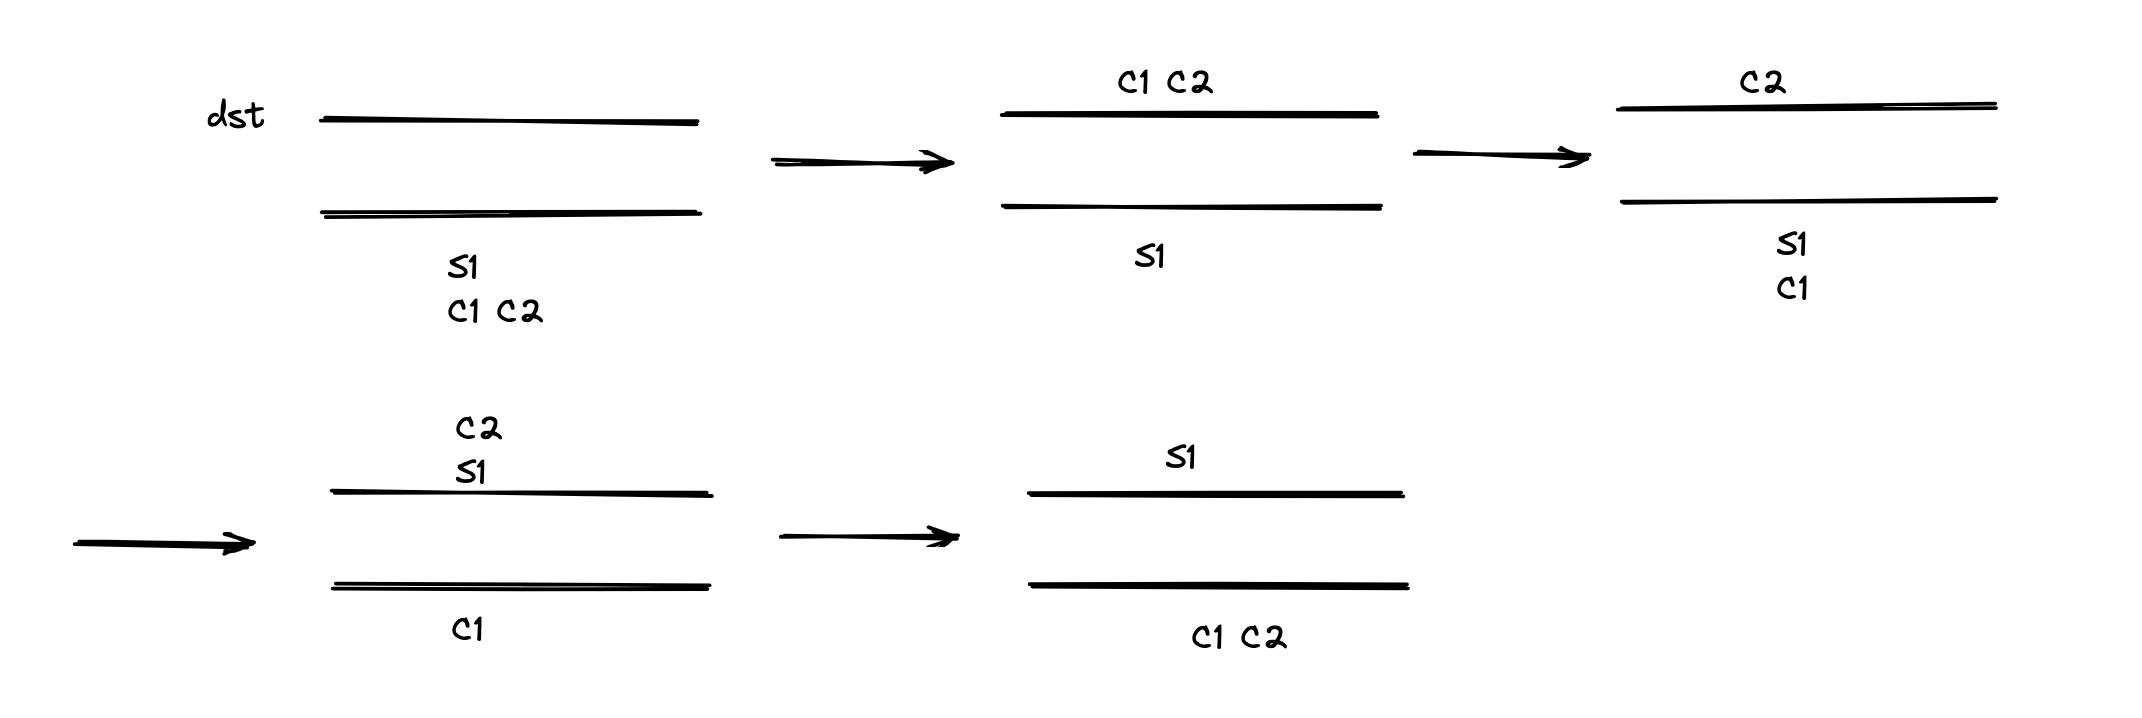
\includegraphics[width=10cm]{../../src/images/hw2-Q2-river.png}
        \caption{一个士兵渡河}  
    \end{figure}

    每多一个士兵,其实就相当于让船多跑四次。

    记 $F(n)$ 为 N 个士兵渡河需要的次数,那么 
    \begin{equation}
        F(n)=\left\{
        \begin{array}{cl}
        4  & n = 1 \\
        F(n-1)+4  & n > 1 \\
        \end{array} \right.
    \end{equation}

    综上,$F(n) = 4n,~ n\ge 1$ 
\end{solution}

\newpage

\begin{problem}
    遍历下面的二叉树,写出遍历顺序(如:abcdef、fedcba): 
    
    a.用前序法 b.用中序法 c.用后序法
\end{problem}
    
\begin{solution}
    \begin{figure}[h]
        \centering
        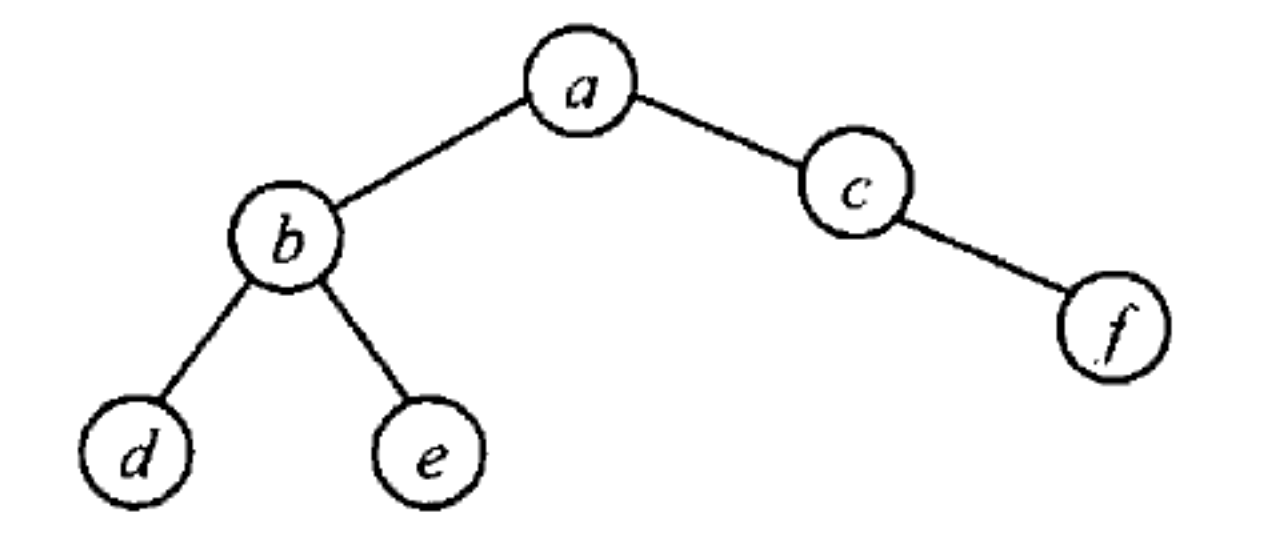
\includegraphics[width=10cm]{../../src/images/hw2-Q3-tree.png}
    \end{figure}

    前序:a b d e c f

    中序:d b e a c f

    后序:d e b f c a
\end{solution}

\newpage 

\begin{problem}
    对于下面的每个列表,从一棵空树开始,通过连续插入它们的元素来构造一棵 AVL 树:
    
    a.1,2,3,4,5,6 
    
    b.6,5,4,3,2,1 
    
    c.3,6,5,1,2,4
\end{problem}


\begin{solution}
    \begin{figure}[h]
        \centering
        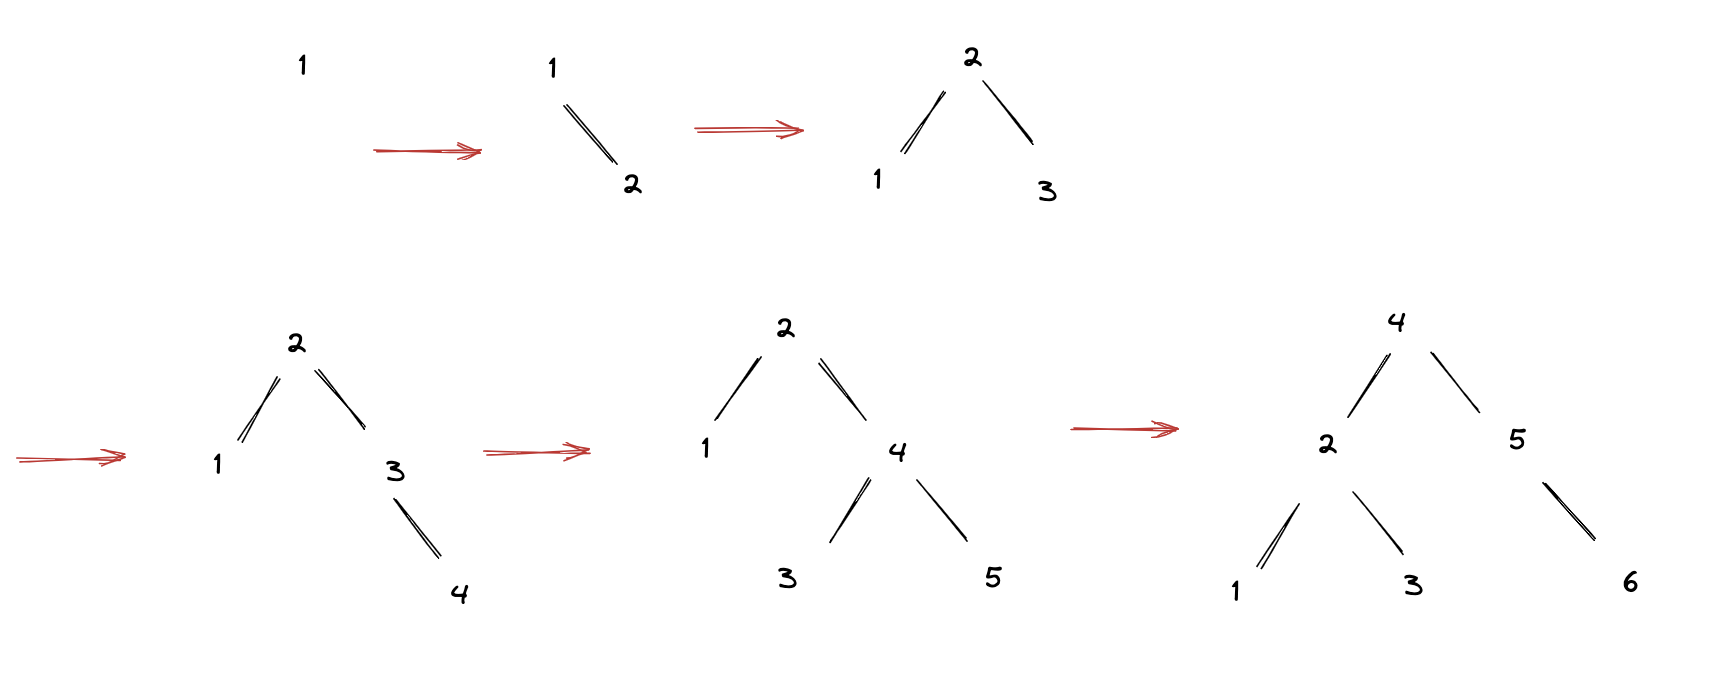
\includegraphics[width=10cm]{../../src/images/hw2-Q4-1.png}
        \caption{a}  
    \end{figure}

    \begin{figure}[h]
        \centering
        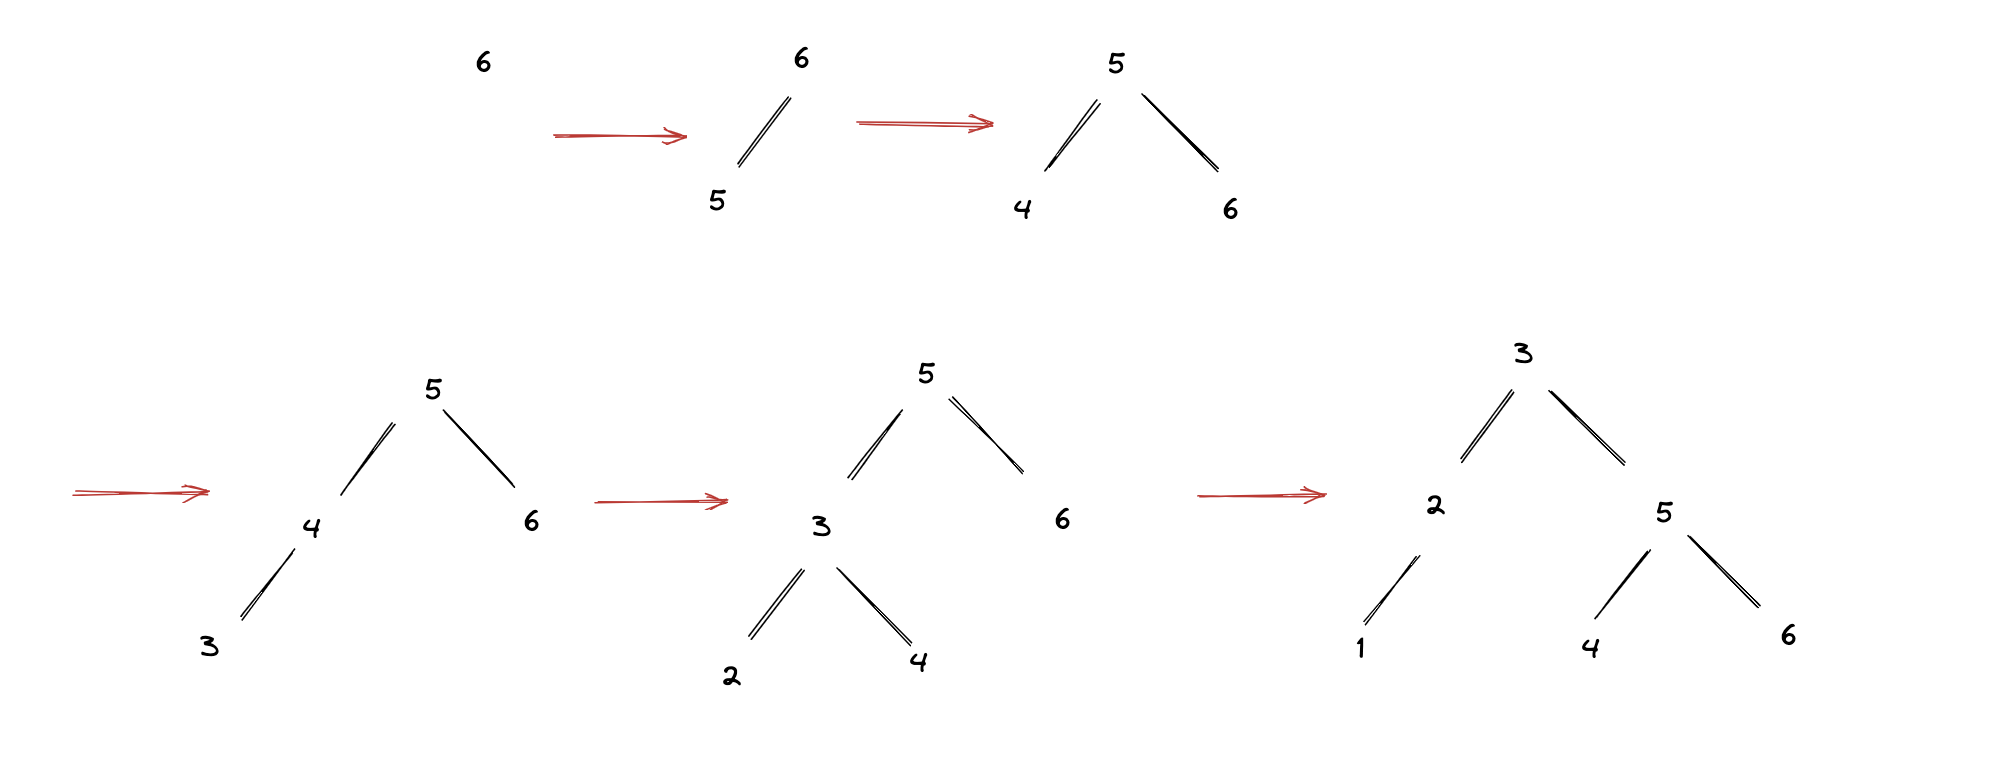
\includegraphics[width=10cm]{../../src/images/hw2-Q4-2.png}
        \caption{b}  
    \end{figure}

    \begin{figure}[h]
        \centering
        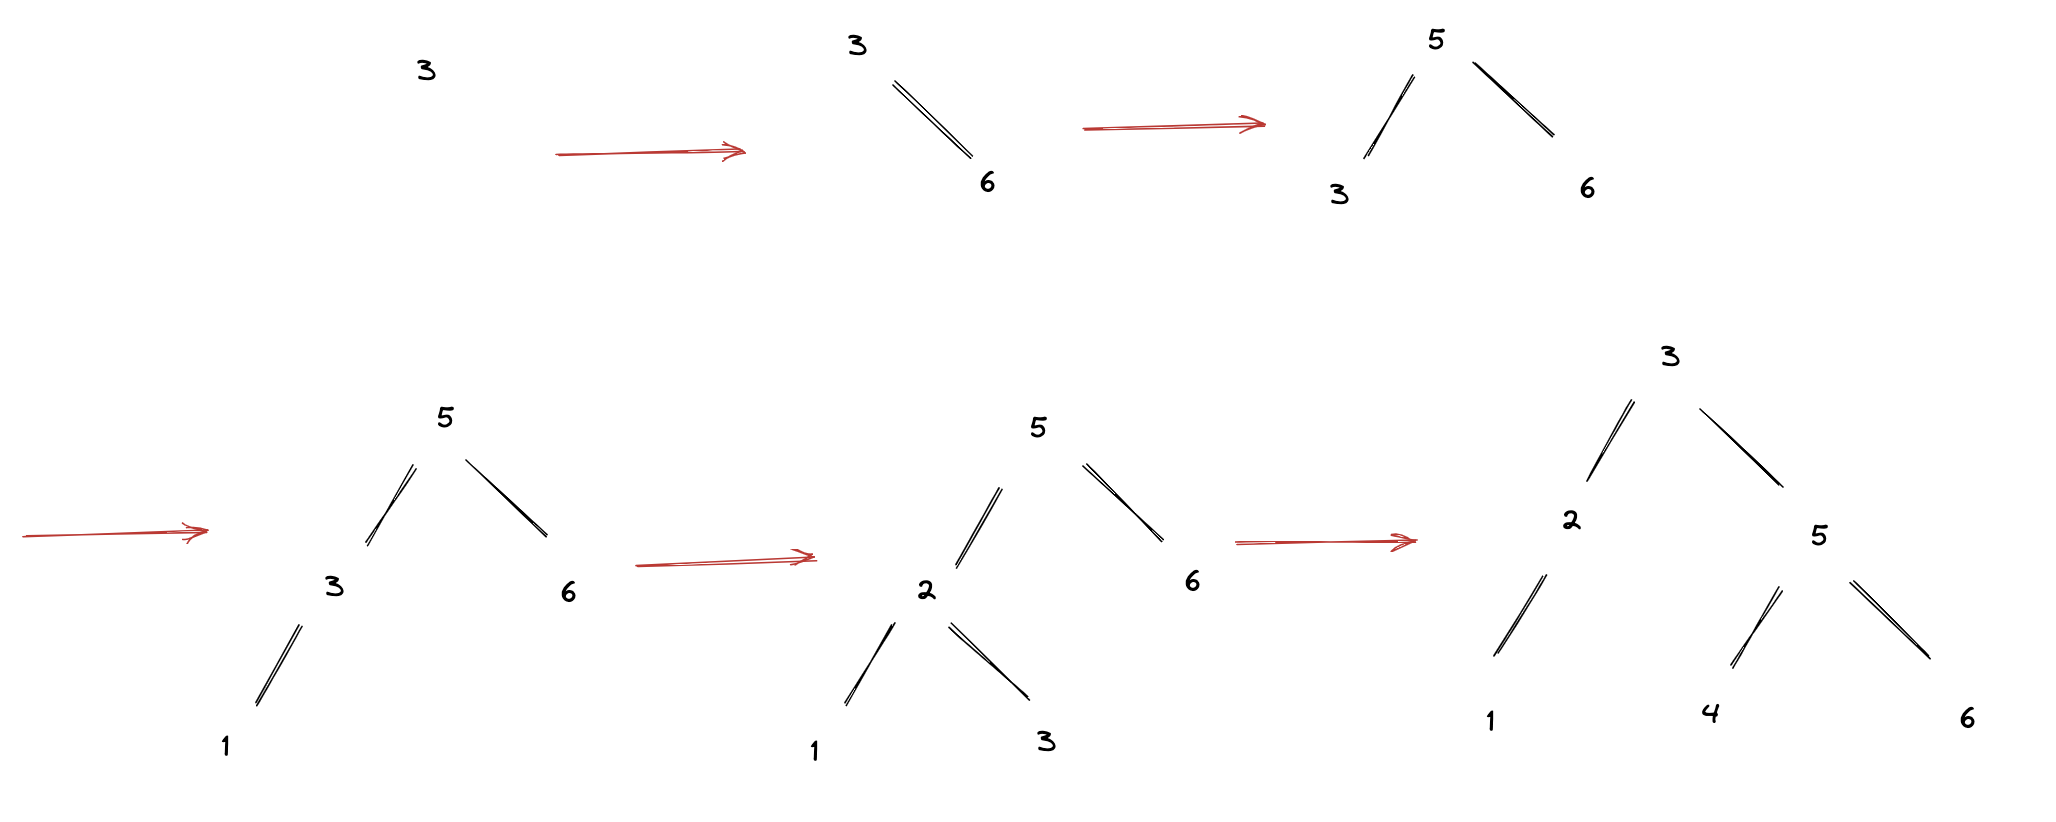
\includegraphics[width=10cm]{../../src/images/hw2-Q4-3.png}
        \caption{c}  
    \end{figure}
\end{solution}

\newpage

\begin{problem}
    吃醋的丈夫谜题 有 n 对夫妇要越过一条河。他们有一条船,但一次最多只能载两个人。为了使情况复杂化,我们假设所有的丈夫都爱吃醋,因此在过河的全过程中, 即使有他人在场,但如果没有本人的陪伴,丈夫也不会允许妻子和其他妻子的丈夫在河的同一岸上。在这种约束下,他们能越过河去吗?
    
    a. 对于 n=2 的情况,求过河的次数
    
    b. 对于 n=3 的情况,求过河的次数
    
    c. 对于任何 $n \ge 4$ 的情况,这个问题有解吗?如果有,请指出他们一共要过多少次河;
如果无解,请解释原因。
\end{problem}

\begin{solution}
    符号说明:

    $A_i$:第 i 对夫妻中的丈夫

    $B_i$:第 i 对夫妻中的妻子

    n 对夫妻要从过河,即从下图中两条直线左侧移动到右侧

    \vspace{2mm}

    a. 过河次数如下图所示:

    \begin{figure}[h]
        \centering
        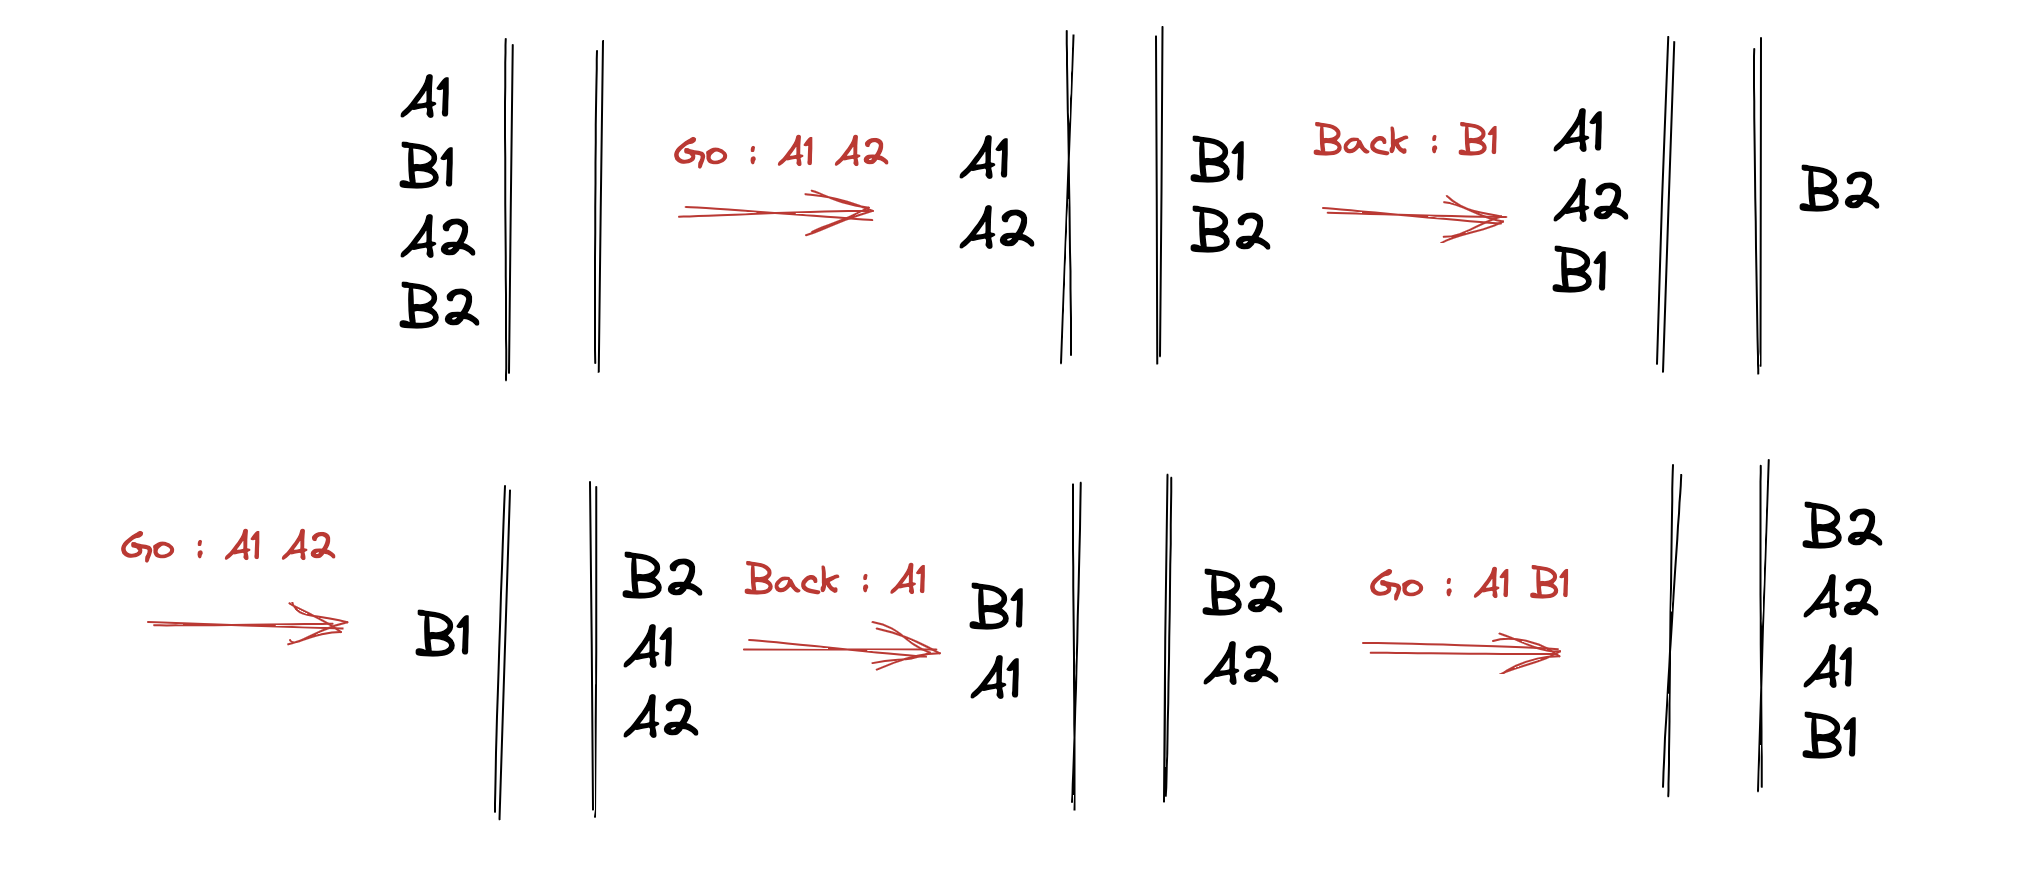
\includegraphics[width=10cm]{../../src/images/hw2-Q5-two-people.png}
        \caption{n=2时的过河次数}
    \end{figure}

    根据图示,过河次数为 5 次。

    b. 过河次数如下图所示:

    \begin{figure}[h]
        \centering
        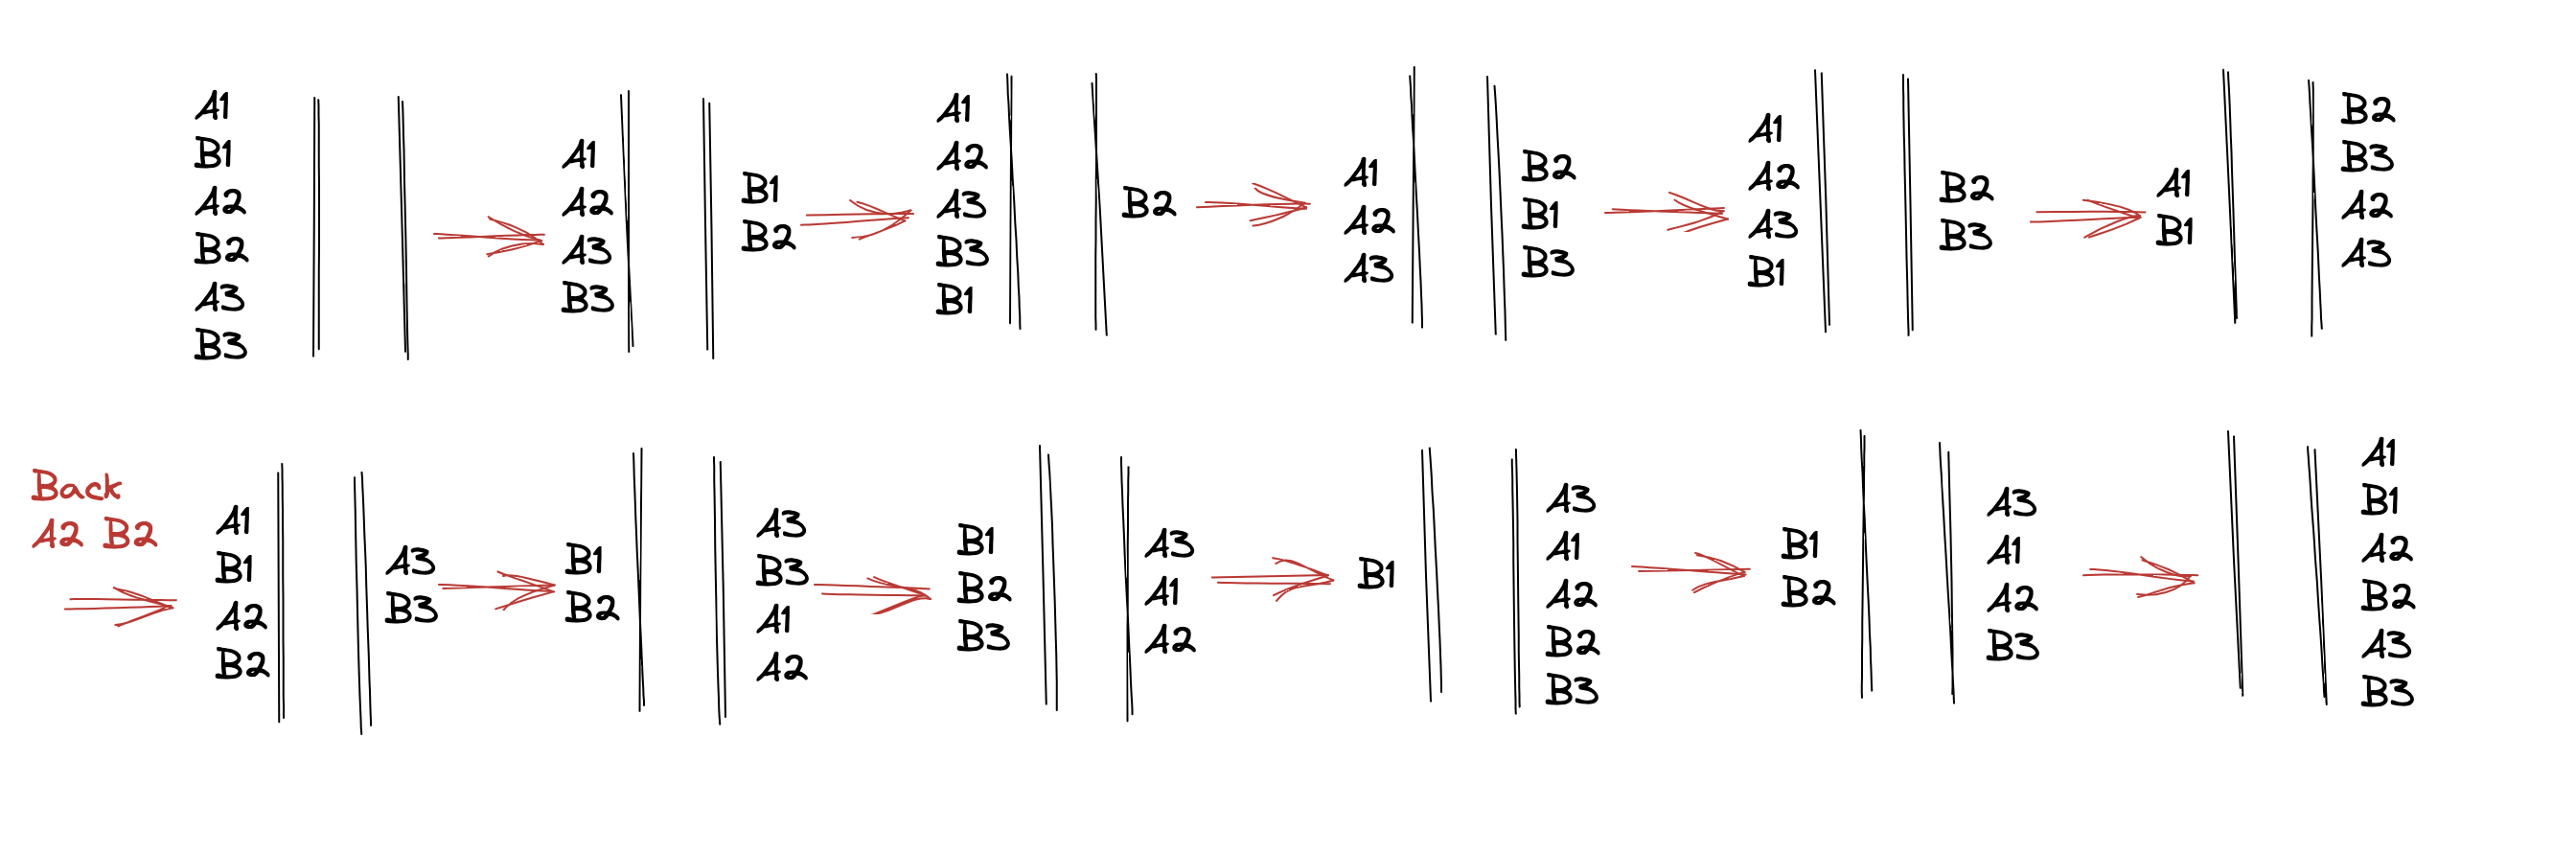
\includegraphics[width=10cm]{../../src/images/hw2-Q5-three-people.png}
        \caption{n=3时的过河次数}
    \end{figure}

    根据图示,过河次数为 11 次。

    c. 无解

    n 对夫妻过河的方法:先让所有妻子过河,再让丈夫一个接一个过河。

    通过穷举法尝试,当 4 对夫妻过河时,会陷入循环,不会产生新的状态,因此无解。
\end{solution}

\end{document}